\chapter{Aplikacja demonstracyjna}
\label{c6:c6}

\section{Opis aplikacji wspomagającej zarządzanie magazynem}
	\subsection{Założenia, wymagania oraz ich realizacja}
		Aplikacja przygotowana jako część praktyczna pracy dyplomowej miała za zadanie
		zobrazować niektóre z funkcji, które powinien spełniać system wspomagający
		zarządzanie gospodarką magazynową. Podstawowym wymaganiem stało się więc
		dostarczenie aplikacji dostępnej z każdego miejsca, posiadającej dostęp
		do centralnej bazy danych oraz wspartej oprogramowaniem umożliwiającym
		zaprogramowanie podstawowych algorytmów. Aplikacja jest dostępna przez interfejs przeglądarki
		internetowej, co daje możliwość korzystania na dowolnej maszynie, bez konieczności
		instalacji skomplikowanego oprogramowania. 
	\subsection{Dostępna funkcjonalność aplikacji}
		Istniejąca funkcjonalność zapewnia:
		\begin{itemize}
			\item Rejestracja nowego przedsiębiorstwa oraz pojedynczego magazynu;
			\item Rejestracje dowolnej ilości stref wydzielonych w magazynie, a także organizowania
			stref w strukturę drzew. Takie rozwiązanie jest elastycznym podejściem, które
			pozwala na przenoszenie ładunków między różnymi strefami, jeśli istnieje taka możliwość, tj.
			gdy strefa C jest, nie koniecznie bezpośrednim, potomkiem strefy A.
			\item Rejestracja nowych klientów: \textbf{dostawców oraz odbiorców}, którzy traktowani są
			zgodnie ze swoją funkcją w misji przedsiębiorstwa, czyli dostawca odpowiedzialny jest
			jedynie za dostawy. Niewykluczona jest sytuacja, gdy ten sam klient, jest zarówno dostawcą, jak
			i odbiorcą. 
		\end{itemize}
	\subsection{Realizacja postulatów aplikacji WMS}
		Aplikacja realizuje postulaty funkcjonalności WMS w obszarach wspomagania gospodarki magazynowej,
		ewidencji towarów, podziału magazyny na logiczne jednostki oraz utrzymania informacji
		o wydaniach / przyjęciach produktów. Odpowiednio wydanie towaru implikuje zmniejszenie stanów
		magazynowych, a przyjęcie zmniejszenie oraz alokację w strefach odkładczych.
\section{Diagramy, zrzuty ekranowe oraz funkcje}
	\subsection{Logowanie do aplikacji przy pierwszym uruchomieniu}
		\begin{figure}[h]
			\centering
			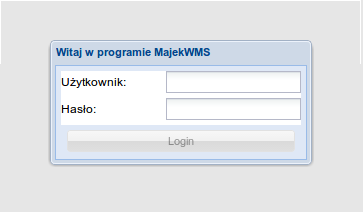
\includegraphics[width=0.99\textwidth]{images/app/login}
			\caption[Aplikacja - Logowanie do programu]{Zrzut ekranu pokazują aplikację w stanie tuż po uruchomieniu}
			\label{c7:fig:app:login}
		\end{figure}
		
	\subsection{Zarządzanie strukturą magazynu}
		\begin{figure}[h]
			\centering
			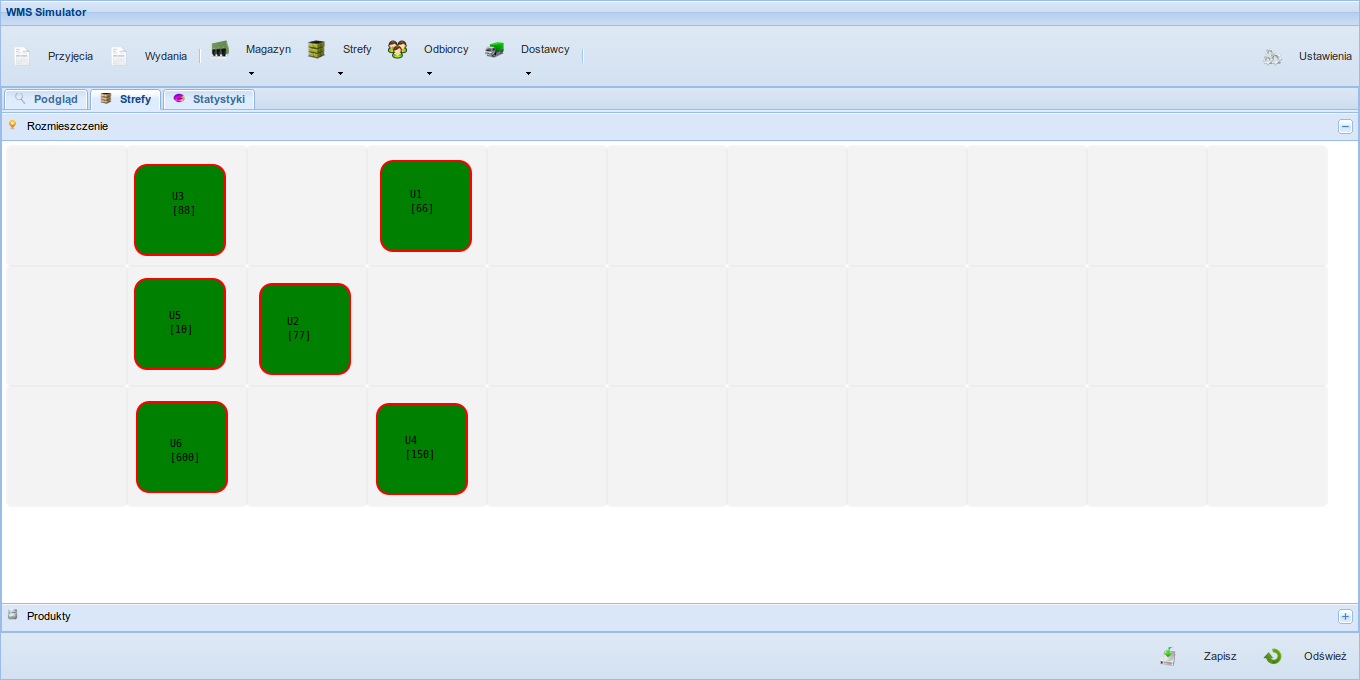
\includegraphics[width=0.99\textwidth]{images/app/unit_preview}
			\caption[Aplikacja - Zarządzania strukturą magazynu]{Zrzut ekranu z widokiem na strukturę magazynu}
			\label{c7:fig:app:unit_preview}
		\end{figure}
		
	\subsection{Zarządzanie klientami - dodawanie, usuwaniu, edycja oraz podgląd}
		\begin{figure}[h]
			\centering
			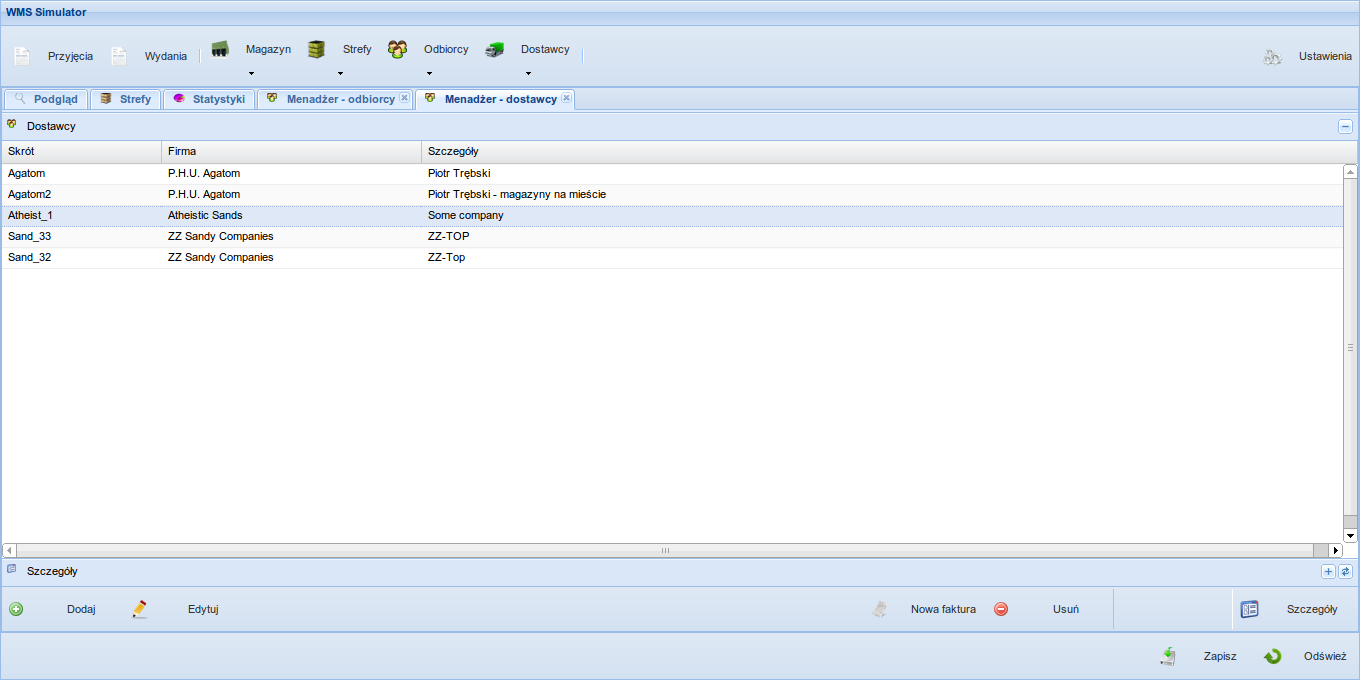
\includegraphics[width=0.99\textwidth]{images/app/supplier_preview}
			\caption[Aplikacja - Dostęp do danych klientów]{Zrzut ekranu z widokiem na dostępnych dostawców}
			\label{c7:fig:app:supplier_preview}
		\end{figure}
		\begin{figure}[h]
			\centering
			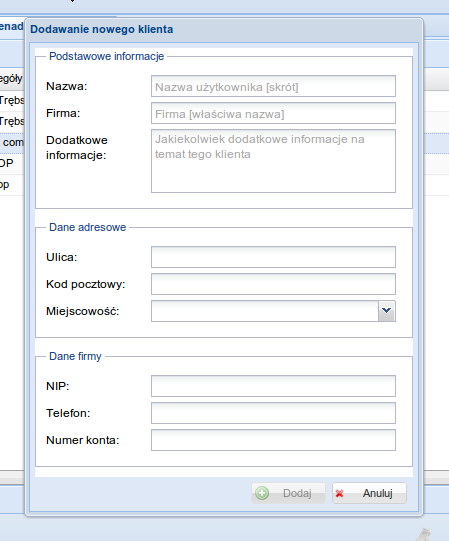
\includegraphics[width=0.6\textwidth]{images/app/new_receipient_dialog}
			\caption[Aplikacja - Dodawania nowego klienta - odbiorcy]{Zrzut ekranu z widokiem na okno dialogowe dla tworzenia nowego odbiorcy}
			\label{c7:fig:app:new_receipient_dialog}
		\end{figure}
		
	\subsection{Wydanie, przyjęcia oraz ewidencja produktów}
		\begin{figure}[h]
			\centering
			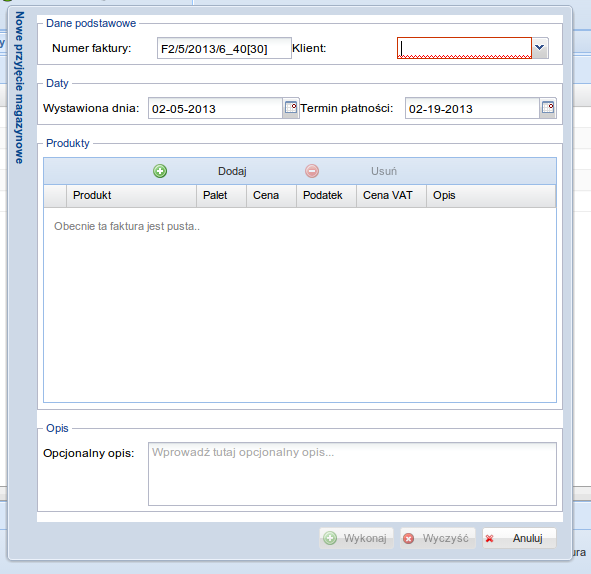
\includegraphics[width=0.99\textwidth]{images/app/new_supply_preview}
			\caption[Aplikacja - Dodanie nowego dokumentu wydania]{Zrzut ekranu z widokiem na kreator nowego wydania magazynowego}
			\label{c7:fig:app:new_supply_preview}
		\end{figure}
		\begin{figure}[h]
			\centering
			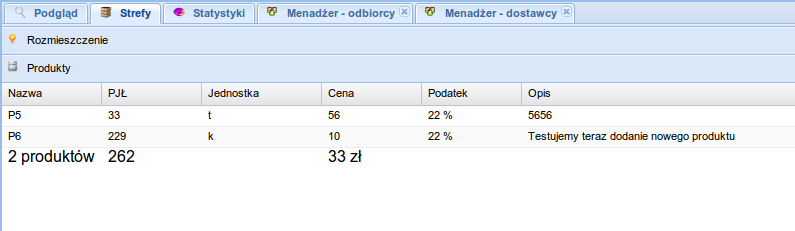
\includegraphics[width=0.8\textwidth]{images/app/unit_products_preview}
			\caption[Aplikacja - Ewidencja towarów w poszczególnych strefach]{Zrzut ekranu z widokiem listy produktów w wybranej strefie}
			\label{c7:fig:app:unit_products_preview}
		\end{figure}